% !TeX program = lualatex
% !TeX encoding = utf8
% !TeX spellcheck = uk_UA
% !BIB program = bibler

\documentclass[onlytextwidth]{beamer}
\usetheme{Electromagnetism}
\usepackage{Electromagnetism}
\usepackage{circuitikz}



%============================================================================
\title[Лекції електрики та магнетизму]{\huge\bfseries Постійний\\ електричний струм}
\subtitle{Лекції з електрики та магнетизму}
\author{Пономаренко С. М.}
\date{}
%============================================================================
\graphicspath{{pictures/}}
\begin{document}
\begin{frame}[plain]
	\maketitle
\end{frame}

% ============================== Слайд ## ===================================
\begin{frame}{Зміст}{}
	\tableofcontents
\end{frame}
% ===========================================================================




%% --------------------------------------------------------
\section{Основні поняття}
%% --------------------------------------------------------




% ============================== Слайд ## ===================================
\begin{frame}{Означення}{Сила та густина струму}\small
	\begin{block}{}\justifying
		\alert{Електричний струм} --- це впорядкований рух зарядів.
	\end{block}
	\begin{block}{}\justifying
		\alert{Силою струму}  називається  заряд, що переноситься через переріз провідника за одиницю
		часу:
		\begin{equation*}
			I = \frac{dq}{dt}.
		\end{equation*}
	\end{block}
	\begin{overprint}
		\onslide<1>
		\begin{block}{}\justifying
			Електричний струм може бути нерівномірно розподілений по поверхні, через яку він
			протікає. Для характеристики розподілу по поверхні вводять \alert{вектор густини струму}
			$\vect{j}$.
			Модуль вектора чисельно дорівнює відношенню сили струму через елементарну площадку,
			розташовану в даній точці перпендикулярно напряму руху носіїв, до її площі:
			\begin{equation*}
				j = \frac{dI}{dS_{\perp}}.
			\end{equation*}
		\end{block}
		\onslide<2>
		\begin{columns}
			\begin{column}{0.7\linewidth}
				\begin{block}{}\justifying
					Знаючи вектор густини струму в кожній точці поверхні $S$, можна знайти силу струму
					через цю поверхню як потік вектора $\vect{j}$:
					\begin{equation*}
						dI = j dS_{\perp}\ \Rightarrow\ \tcbhighmath{ I = \iint\limits_S \vect{j}\cdot
							d\vect{S}.}
					\end{equation*}
				\end{block}
			\end{column}
			\quad
			\begin{column}{0.3\linewidth}\centering
				\begin{tikzpicture}[>=latex, every node/.style={font=\scriptsize}, scale=0.7,
		transform shape]
	\draw[ball color=blue!5] (0,0) to[bend left] ++(2,1.9)  to[bend left] ++(2,-2)
	to[bend right]
	++(-2, -1)  to[bend
		right] cycle;
	\draw[->, jfield] (0.2, 0.2) -- ++(80:1.5);
	\draw[->, jfield] (0.8, 1) -- ++(80:1.5);
	\draw[->, jfield] (1.6, 1.6) -- ++(80:1.5);

	\draw[->, jfield] (1.2, 0) -- ++(75:1.5);
	\draw[->, jfield] (2.2, 0.8) coordinate (A) -- ++(70:2) coordinate (B)
	node[above] {$\vect{j}$};
	\draw[->, jfield] (3, 1.2) -- ++(70:1.5);

	\draw[->, jfield] (2, -0.4) -- ++(45:1.5);
	\draw[->, jfield] (2.8, 0) -- ++(45:1.5);
	\draw[->, jfield] (3.8, 0.2) -- ++(35:1.5);

	\draw[fill=gray!50, opacity=0.5] (A) circle(0.5 and 0.15);
	\draw[dashed] (A) ++(70:1.5) circle(0.5 and 0.15);
	\draw[->, green!50!black, thick] (A) -- ++(90:0.5) node[above, text=black]
	{$\vect{n}$};
	\draw[densely dashed] (A) ++(180:0.5) -- ++(70:1.5);
	\draw[densely dashed] (A) ++(0:0.5) -- ++(70:1.5);
\end{tikzpicture}
			\end{column}
		\end{columns}
	\end{overprint}
\end{frame}
% ===========================================================================

% ============================== Слайд ## ===================================
\begin{frame}{Означення}{Густина струму та густина заряду}
	\begin{block}{}\justifying
		Середню швидкість впорядкованого руху носіїв заряду під дією електричного поля в провіднику
		називають \alert{дрейфовою швидкістю}.
	\end{block}

	%\begin{block}{}\justifying\scriptsize
	%
	%\end{block}

	\begin{columns}
		\begin{column}{0.7\linewidth}
			\begin{block}{}\justifying\scriptsize
				Візьмемо площадку $dS$ на шляху носіїв, перпендикулярний дрейфовій швидкості. За час $dt$ цю
				площадку перетнуть носії, що перебувають у циліндрі об'ємом $dV = udt\ S$ . Їхнє
				число дорівнює
				$dN = ndV$, а перенесуть вони сумарний заряд $dq = e dN = enudt\ S$. За одиницю часу
				через одиничну площадку пройде заряд:
				\begin{equation*}
					j = \frac{dq}{dt}\frac1S = enu = \rho u
				\end{equation*}
			\end{block}
		\end{column}
		\begin{column}{0.3\linewidth}\centering
			\begin{tikzpicture}[
	electron/.pic={
			\begin{scope}[opacity=0.7]
				\node[scale=0.2,circle, ball color=red, inner sep=0, minimum
					size=0.1cm,
					text=white] (e) at
				(0,0)
				%{\tikz\draw[white, thick](0,0)--++(0.2,0);}
				{$+$};
			\end{scope}
			\draw[-latex, jfield, line width=0.1pt] (e) -- ++(0.25, 0);
		}
]
	\pgfmathsetmacro{\r}{1}
	\pgfmathsetmacro{\l}{2}
	\pgfmathsetseed{6}
	\draw[fill=red!10, thin] (0,0) circle(0.2 and \r);
	\draw[fill=red!10, thin] (0, \r) -- ++(\l, 0) coordinate (A) arc[x
			radius=0.2, y
			radius=\r, start angle=90, delta  angle=-180] -- node[below] {$udt$} ++(-\l, 0)
	arc[x radius=0.2, y radius=\r, start angle=-90, delta  angle=180];
	\draw[dashed, thin] (A) arc[x radius=0.2, y radius=\r, start angle=90, delta
			angle=180];
	\foreach \x in {-0.3,0,...,2.5}
		{
			\foreach \y in {-1.3,-1.0,...,1.3}{
					\pic[rotate={random(-30,30)}] at ({0.75*\x+ 0.2*rnd},
					{0.75*\y+0.2*rnd})
					{electron};
				}
		}
	\path (0, -0.01) node[text=white,
		scale=1.1, font=\bfseries] {$S$} node[] {$S$} ;
\end{tikzpicture}
		\end{column}
	\end{columns}
	\begin{block}{}
		У векторному вигляді
		\begin{equation*}
			\vect{j} = \rho\vect{u}.
		\end{equation*}
	\end{block}
\end{frame}
% ===========================================================================




%% --------------------------------------------------------
\section{Природа носіїв заряду}
%% --------------------------------------------------------




% ============================== Слайд ## ===================================
\begin{frame}{Природа носіїв струму в металах}{Досліди Толмена та Стюарта}\scriptsize
	\begin{block}{}\justifying
		У 1916 р. американський фізик Р. Толмен (1881-1948) і шотландський фізик Т. Стюарт виконали
		кількісні виміри, які неспростовно довели, що струм у металевих провідниках зумовлений рухом
		вільних електронів.
	\end{block}
	%\begin{onlyenv}<1>
	\begin{columns}
		\begin{column}{0.65\linewidth}
			\begin{block}{}\justifying
				У цих дослідах котушку з великим числом витків тонкого дроту підключали до гальванометра і
				приводили в швидке обертання навколо своєї осі. Під час різкого гальмування котушки в колі
				виникав короткочасний струм, зумовлений інерцією носіїв заряду. За напрямком відхилення
				стрілки гальванометра було встановлено, що \alert{електричний струм створюють негативно
					заряджені частинки}. При цьому експериментально був отриманий питомий заряд носіїв $q/m$
				близький до питомого заряду електрона, отриманого з інших дослідів. Так було експериментально
				доведено, що носіями вільних зарядів у металах є електрони.
			\end{block}
		\end{column}
		\hfill
		\begin{column}{0.3\linewidth}\centering
			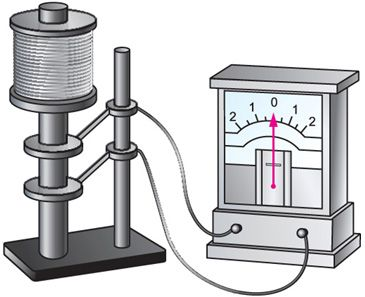
\includegraphics[width=\linewidth]{exptommstuart}
			\begin{block}{}\centering
				Установка Толмена і Стюарта
			\end{block}
		\end{column}
	\end{columns}
	\begin{block}{}
		\href{https://www.youtube.com/watch?v=nVwquffMk44}{\color{blue}Відеодемотнстрація дослідів}
	\end{block}
	%\end{onlyenv}
	%\begin{onlyenv}<2>
	%У досліді котушка, що обертається, має кутову швидкість \( \omega \). Струм, що виникає
	%\begin{equation*}
	%j = n e u S = n e \omega r S
	%\end{equation*}
	%
	%З закону Ома
	%\begin{equation*}
	%E = \rho j = \frac{\rho I}{S} = \rho n e \omega r.
	%\end{equation*}
	%
	%Сила інерції, що діє на електрони:
	%\begin{equation*}
	%F = ma = eE = m \omega^2 r.
	%\end{equation*}
	%Звідки питомий заряд:
	%\begin{equation*}
	%\frac{e}{m} = \frac{\omega^2 r}{E} = \frac{\omega}{\rho n e}
	%\end{equation*}
	%\pgfkeys{/pgf/fpu}
	%\pgfmathparse{523.6/(1.68e-8*8.5e28*1.6e-19)}
	%\pgfkeys{/pgf/fpu=false}
	%В досліді частота обертання була $ 5000 $~об/хв. Дріт був мідний в якому концентрація електронів
	%$n
	%= 8.5\cdot 10^{28}$~м${}^{-3}$, питомий опір міді $\rho = 1.68\cdot 10^{-8}$~Ом$\cdot$м, звідки:
	%$e/m = \pgfmathprintnumber\pgfmathresult$
	%\end{onlyenv}
\end{frame}
% ===========================================================================




% ============================== Слайд ## ===================================
\begin{frame}{Задачі}{}
	\begin{exampleblock}{Швидкість носіїв струму}\justifying\scriptsize
		Срібним дротом з перерізом $1$~мм${^2}$ проходить струм сили $1$~А. Обчисліть середню
		швидкість упорядкованого руху електронів у цьому дроті, вважаючи, що кожен атом срібла дає
		один вільний електрон. Густина срібла дорівнює $10.5\cdot 10^3$кг/м${^3}$, його відносна
		атомна маса дорівнює $108$. Постійна Авогадро $N_A = 6.02\cdot 10^{23}$~моль${}^{-1}$.
		Обчисліть теплову швидкість електронів при $T = 300$~K.
	\end{exampleblock}
	\begin{block}{}\justifying\scriptsize
		Струм
		\begin{equation*}
			I = jS = enuS
		\end{equation*}
		Концентрація електронів --- це число електронів в одиниці об'єму, а число електронів дорівнює числу
		атомів срібла, бо один атом віддає один електрон:
		\begin{equation*}
			\rho = \frac{m_{\ce{Ag}}N}{V} = m_{\ce{Ag}}n, \ \Rightarrow\ n= \frac{\rho}{m_{\ce{Ag}}} = \rho
			\frac{\mu}{N_A}.
		\end{equation*}
		Середня швидкість:
		\begin{equation*}
			\pgfkeys{/pgf/fpu}
			\pgfmathparse{1*108e-3/(1e-19*10.5e3*6.02e23*(1e-3)^2)*1e3}
			\pgfkeys{/pgf/fpu=false}
			u = \frac{I}{enS} = \frac{I\mu}{e\rho N_A S} = \pgfmathprintnumber[precision=2]\pgfmathresult\
			\text{мм/с}.
		\end{equation*}
		Теплова швидкість --- це середні квадратична швидкість:
		\begin{equation*}
			\pgfkeys{/pgf/fpu}
			\pgfmathparse{sqrt(3*1.38e-23*300/9.1e-31)}
			\pgfkeys{/pgf/fpu=false}
			v_T = \sqrt{{3kT}/{m_e}} = \pgfmathprintnumber[precision=2]\pgfmathresult\
			\text{м/с}.
		\end{equation*}
	\end{block}
\end{frame}
% ===========================================================================




%% --------------------------------------------------------
\section{Закон збереження заряду}
%% --------------------------------------------------------



% ============================== Слайд ## ===================================
\begin{frame}{Закон збереження заряду}{}\small
	\begin{columns}
		\begin{column}{0.7\linewidth}
			\begin{block}{}\justifying
				Нехай в деякому провідному середовищі, струм, який витікає через поверхню $S$ дорівнює $I =
					\oiint\limits_S  \vect{j} d\vect{S}$. Оскільки струм --- це рух зарядів, то заряд  в об'ємі $V$
				має заряд зменшується з часом:
				\begin{equation*}
					\oiint\limits_S \vect{j} d\vect{S} = -\frac{d}{dt} \iiint\limits_V \rho dV
				\end{equation*}
			\end{block}
		\end{column}\hfill
		\begin{column}{0.3\linewidth}
			\begin{tikzpicture}[>=latex,
		scale=0.75, transform shape,
		pencildraw/.style={ %
				decorate,
				decoration={random steps,segment length=3pt,amplitude=2pt}
			}]

	\pgfmathsetseed{10}
	\fill[pencildraw, red!20] (-2, -2) rectangle (2,2);
	\draw[fill=red!30, name path=metall, smooth, densely dashed, draw=gray!50] plot
		[smooth
			cycle,
			samples=8,domain={1:10}]
	(\x*360/10+5*rnd:0.5cm+1cm*rnd);
	\uncover<1>{
		\foreach \x in {1,...,10} {
				\draw[->, line width=1pt, jfield] (0,0)
				++(\x*360/10+5*rnd:0.5cm+1cm*rnd) --
				++(\x*360/10+5*rnd:0.7cm+1cm*rnd);
			}
	}
	\uncover<2>{
		\foreach \y in {-3,...,3}{
				\draw[jfield, midarrow] plot[domain=0.5:3] ({\x-2},
				0.2*\y+0.05*\y*\x^2);
			}
	}
	\path (0, 0) node[text=white,
		scale=1.1, font=\bfseries] {$V$} node[] {$V$} ;
	\path (135:1.1) node[text=white,
		scale=1.1, font=\bfseries] {$S$} node[] {$S$} ;
\end{tikzpicture}
		\end{column}
	\end{columns}
	\begin{overprint}
		\onslide<1>
		\begin{block}{}\justifying
			Це співвідношення називають \alert{рівнянням неперервності}. Воно є \alert{вираженням закону
				збереження електричного заряду}.
			\bigskip

			В диференціальній формі (використовуючи теорему Остро\-градсь\-кого-Гаусса):
			\begin{equation*}
				\tcbhighmath{\divg\vect{j} = - \frac{\partial\rho}{\partial t}.}
			\end{equation*}
		\end{block}
		\onslide<2>
		\begin{block}{}\justifying
			У \alert{стаціонарному випадку}, коли $\partial\rho/\partial t = 0$, рівняння  набуває вигляду:
			\begin{equation*}
				\oiint\limits_S \vect{j} d\vect{S} = 0,\ \text{або}\ \divg\vect{j} = 0.
			\end{equation*}
			\alert{Дана рівність означає, що з об'єму $V$, обмеженого замкненою поверхнею $S$, витікає така ж
				сама кількість заряду, що і втікає в цей об'єм.}
		\end{block}
	\end{overprint}
\end{frame}
% ===========================================================================



% ============================== Слайд ## ===================================
\begin{frame}{Закон Ома}{}
	\begin{block}{}\justifying
		Георг Ом 1827 року експериментально встановив, що сила струму $I$, який протікає однорідним
		металевим провідником, у якому не діють сторонні сили, пропорційна напрузі $U$ на кінцях
		провідника:
		\begin{equation*}
			I = \frac{U}{R}.
		\end{equation*}
	\end{block}
	\begin{block}{}\justifying
		Опір $R$ залежить від форми і розмірів провідника, від його матеріалу і температури, а також
		від розподілу струму по провіднику. У найпростішому випадку однорідного циліндричного
		провідника опір:
		\begin{equation*}
			R = \rho \frac{l}{S}.
		\end{equation*}
	\end{block}
\end{frame}
% ===========================================================================



%% --------------------------------------------------------
\section{Про одиниці вимірювання}
%% --------------------------------------------------------


% ============================== Слайд ## ===================================
\begin{frame}{Про одиниці вимірювання}{}
	\begin{block}{}\justifying
		Одиниця вимірювання опору в гауссовій системі:
		\begin{equation*}
			[I] = \frac{\text{Фр}}{\text{с}}, [U] = \frac{\text{Фр}}{\text{см}}, \Rightarrow\ [R] =
			\frac{\text{с}}{\text{см}}
		\end{equation*}
		Опір в системі СГС має розмірність оберненої швидкості. Питомий опір відповідно:
		\begin{equation*}
			[\rho] = [R]\frac{[S]}{[l]} = \frac{\text{с}}{\text{см}} \frac{\text{см}^2}{\text{см}}
			= \text{с}
		\end{equation*}
		У гаусовій системі одиниць питомий опір $\rho$ вимірюється в секундах (с).
		Електрична провідність $\lambda$ має розмірність, обернену часу с${^{-1}}$.
	\end{block}
\end{frame}
% ===========================================================================




%% --------------------------------------------------------
\section{Закон Ома}
%% --------------------------------------------------------


% ============================== Слайд ## ===================================
\begin{frame}{Закон Ома}{Диференціальна форма}\small
	\begin{columns}
		\begin{column}{0.7\linewidth}
			\begin{block}{}\justifying
				Виділимо в околиці деякої точки провідного середовища елементарний циліндричний об'єм з
				твірними, паралельними вектору $\vect{j}$.
			\end{block}
		\end{column}
		\hfill
		\begin{column}{0.25\linewidth}\centering
			\begin{tikzpicture}[>=latex,
		scale=0.75, transform shape,
		pencildraw/.style={ %
				decorate,
				decoration={random steps,segment length=3pt,amplitude=2pt}
			}]
	\pgfmathsetmacro{\r}{0.55}
	\pgfmathsetmacro{\l}{2}
	\fill[pencildraw, red!20] (-2, -1) rectangle (2,1);
	\draw[fill=red!10, thin] (-1,0) circle(0.2 and \r);
	\draw[fill=red!10, thin] (-1, \r) -- ++(\l, 0) coordinate (A) arc[x
			radius=0.2, y radius=\r, start angle=90, delta  angle=-180] -- ++(-\l,
	0) arc[x radius=0.2, y radius=\r, start angle=-90, delta  angle=180];
	\draw[dashed, thin] (A) arc[x radius=0.2, y radius=\r, start angle=90,
			delta angle=180];
	\foreach \y in {-0.8, -0.5,..., 0.8}
		{
			\draw[->, jfield] (-1.8, \y) -- ++(3.6,0);
		}
	\path (-1.5, 0) node[text=white,
		scale=1.1, font=\bfseries] {$dS$} node[] {$dS$} ;
	\path (0, -1) node[text=white,
		scale=1.1, font=\bfseries] {$dl$} node[] {$dl$} ;
\end{tikzpicture}
		\end{column}
	\end{columns}
	\begin{block}{}\justifying
		Якщо поперечний переріз циліндра $dS$, а його довжина $dl$, то можна записати для такого
		елементарного циліндра:
		\begin{equation*}
			jdS = \frac{Edl}{\rho \frac{dl}{dS}} = \frac1\rho EdS.
		\end{equation*}
		і після відповідних скорочень отримаємо, вже у векторному вигляді:
		\begin{equation*}
			\tcbhighmath{\vect{j} = \frac1\rho \Efield} = \lambda \Efield
		\end{equation*}
		де $\lambda = 1/\rho$ --- питома електропровідність середовища.
	\end{block}
\end{frame}
% ===========================================================================


%% --------------------------------------------------------
\subsection{Теорія провідності металів Друде}
%% --------------------------------------------------------



% ============================== Слайд ## ===================================
\begin{frame}{Теорія провідності металів Друде}{}\small
	\begin{block}{}\justifying\scriptsize
		У 1900 році Пауль Друде запропонував просту теорію, що пояснює провідність металів. Ця теорія
		доволі проста і якісно застосовується для оцінки провідності.
	\end{block}
	\begin{block}{}\justifying
		Розглянемо рух електрона в постійному однорідному полі $\Efield$. Рівняння руху має вигляд:
		\begin{equation*}
			\vect{a} = \vect{F} / m_e = e\Efield / m_e.
		\end{equation*}
	\end{block}

	\begin{columns}
		\begin{column}{0.3\linewidth}\centering
			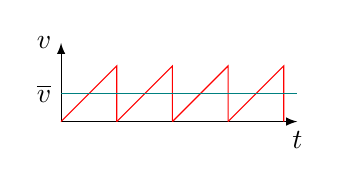
\begin{tikzpicture}[>=latex]
	\draw[->] (0,0) -- ++(3, 0) node[below] {$t$};
	\draw[->] (0,0) -- ++(0, 1) node[left] {$v$};
	\foreach \i in {0,...,3}{
			\draw[red, shift={({\i*cos(45)}, 0)}] (0,0) -- (45:1) -- ++(0, {-sin(45)});
		}
	\draw[teal] (0,{0.5*sin(45)}) node[left, text=black] {$\overline{v}$} -- ++(3,
	0);
\end{tikzpicture}
		\end{column}
		\begin{column}{0.65\linewidth}
			\begin{block}{}\justifying\scriptsize
				Якщо початкова швидкість електрона була нульовою, то до зіткнення з розсіювальним центром
				вона змінюється за законом ${v} = {a} t$. Після зіткнення швидкість обертається в
				середньому в нуль, і починається новий цикл прискорення.
			\end{block}
		\end{column}
	\end{columns}
	\begin{block}{}\justifying
		Якщо час вільного пробігу дорівнює $\tau$, то середня швидкість упорядкованого руху
		електрона
		від зіткнення до зіткнення становитиме
		\begin{equation*}
			\vect{u} = \overline{\vect{v}} = \frac12 \frac{e\Efield \tau}{m_e}.\
			\Rightarrow\ \vect{j} = en\vect{u} = \frac{ne^2\tau}{2m_e}\Efield, \
			\Rightarrow\ \lambda = \frac{ne^2\tau}{2m_e}.
		\end{equation*}
	\end{block}
\end{frame}
% ===========================================================================


%% --------------------------------------------------------
\subsection{Температурна залежність опору}
%% --------------------------------------------------------



% ============================== Слайд ## ===================================
\begin{frame}{Температурна залежність опору}{}
	\begin{columns}
		\begin{column}{0.3\linewidth}\centering
			\begin{figure}
				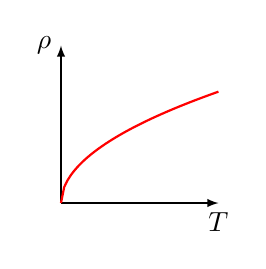
\begin{tikzpicture}[>=latex]
	\draw[->] (0,0) -- ++(2, 0) node[below] {$T$};
	\draw[->] (0,0) -- ++(0, 2) node[left] {$\rho$};
	\draw[domain=0:2, red, thick, samples=50] plot (\x, {sqrt(\x)});
\end{tikzpicture}
				\caption{Теорія Друде}
			\end{figure}
		\end{column}
		\begin{column}{0.3\linewidth}\centering
			\begin{figure}
				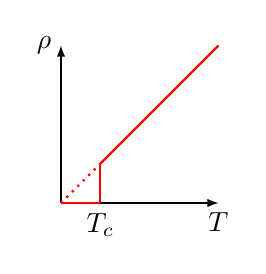
\begin{tikzpicture}[>=latex]
	\draw[->] (0,0) -- ++(2, 0) node[below] {$T$};
	\draw[->] (0,0) -- ++(0, 2) node[left] {$\rho$};
	\draw[domain=0:0.5, red, thick] plot (\x, {0*\x});
	\draw[domain=0.5:2, red, thick] plot (\x, {\x});
	\draw[red, thick] (0.5, 0) node[below, text=black] {$T_c$} --++ (0,0.5);
	\draw[red, thick, dotted] (0, 0)  --++ (0.5,0.5);
\end{tikzpicture}
				\caption{Експеримент}
			\end{figure}
		\end{column}
		\begin{column}{0.3\linewidth}
			\begin{equation*}
				\rho = \rho_{0}\left[ 1 + \alpha T \right] .
			\end{equation*}
			\begin{equation*}
				\rho = \rho_{20}\left[ 1 + \alpha(t - 20) \right] .
			\end{equation*}
		\end{column}
	\end{columns}
	\begin{table}[h]\scriptsize
		\centering
		\caption{Питомий опір металів при $20^\circ$C}
		\begin{tblr}
			{
			colspec = {Q[l, m]Q[c, m]Q[c, m]},
			hlines,
			vlines,
			row{1} = {c, bg=cyan, fg=white, font=\bfseries},
			}
			Метал              & $\rho$, $\mathbf{\rho}$ ($10^{-8}\ \text{Ом} \cdot \text{м}$) & $\alpha$, $10^{-3}\ 1/{}^\circ$C \\
			Мідь (\ce{Cu})     & 1.68                                                          & 4.3                              \\
			Алюміній (\ce{Al}) & 2.82                                                          & 4.2                              \\
			%            Золото   (\ce{Au}) & 2.44 & 4.0  \\
			%            Срібло   (\ce{Ag}) & 1.59 & 4.1  \\
			Залізо   (\ce{Fe}) & 9.71                                                          & 6.0                              \\
			Нікель   (\ce{Ni}) & 6.84                                                          & 6.5                              \\
			%            Платина  (\ce{Pt}) & 10.6 & 3.9  \\
			Вольфрам (\ce{W})  & 5.65                                                          & 5.0                              \\
		\end{tblr}
	\end{table}
\end{frame}
% ===========================================================================


%% --------------------------------------------------------
\subsection{Розподіл зарядів в провіднику}
%% --------------------------------------------------------




% ============================== Слайд ## ===================================
\begin{frame}{Розподіл зарядів в провіднику}{}
	\begin{block}{Об'ємні заряди}\justifying
		Якщо по однорідному ($\lambda = \const$) провіднику тече постійно струм $\divg\vect{j} = 0$:
		\begin{equation*}
			\divg\vect{j} = \lambda\divg\Efield = \lambda 4\pi \rho = 0\ \Rightarrow\ \rho = 0.
		\end{equation*}
		Це означає, що при протіканні струму по однорідному провіднику в його об'ємі нема заряду $\rho
			= 0$.
	\end{block}

	\begin{block}{Поверхневі заряди}
		\begin{columns}
			\begin{column}{0.7\linewidth}\justifying
				На поверхні провідника, по якому тече постійний електричний струм, є електричні заряди.
				Вони і є джерелами електричного поля, яке існує в провіднику і забезпечує наявність
				постійного струму.
			\end{column}
			\hfill
			\begin{column}{0.25\linewidth}\centering
				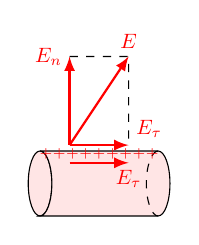
\begin{tikzpicture}[>=latex,
		scale=0.75, transform shape]
	\pgfmathsetmacro{\r}{0.55}
	\pgfmathsetmacro{\l}{2}
	\draw[fill=red!10, thin] (-1,0) circle(0.2 and \r);
	\draw[fill=red!10, thin] (-1, \r) -- ++(\l, 0) coordinate (A) arc[x
			radius=0.2, y radius=\r, start angle=90, delta  angle=-180] -- ++(-\l,
	0) arc[x radius=0.2, y radius=\r, start angle=-90, delta  angle=180];
	\draw[dashed, thin] (A) arc[x radius=0.2, y radius=\r, start angle=90,
			delta angle=180];
	\draw[->, red, thick] (-0.5,0.35) -- ++(1,0) node[below] {$E_{\tau}$};
	\draw[->, red, thick] (-0.5,0.65) -- ++(1,0) coordinate (Et)  node[above right]
		{$E_{\tau}$} ;
	\draw[->, red, thick] (-0.5,0.65) -- ++(0,1.5) coordinate (En) node[left] {$E_n$};
	\draw[->, red, thick] (-0.5,0.65) -- ++({atan(1.5)}:{1/(cos(atan(1.5)))})
	coordinate (E) node[above] {$\vect{E}$};
	\draw[dashed] (En) -- (E) -- (Et);
	\foreach \x in {-1, -0.75,..., 1} {
			\node[inner sep=0, text=red, font=\scriptsize] at ({0.9*\x}, {\r-0.05}) {$+$};
		}
\end{tikzpicture}
			\end{column}
		\end{columns}
	\end{block}
\end{frame}
% ===========================================================================


%% --------------------------------------------------------
\subsection{Сторонні сили}
%% --------------------------------------------------------




% ============================== Слайд ## ===================================
\begin{frame}{Сторонні сили}{}
	\begin{columns}
		\begin{column}{0.4\linewidth}\centering
			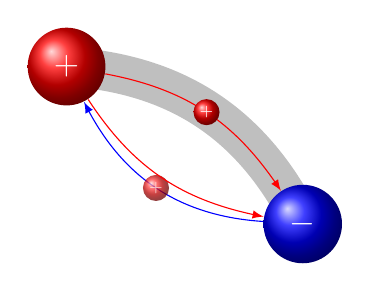
\begin{tikzpicture}[>=latex]
	\draw[gray!50, line width=0.5cm] (-1, +1) coordinate (+) to [bend left] (+2, -1) coordinate (-);
	\node[circle, ball color = red, inner sep=0.2cm,  text=white, font=\bfseries\large]  (P) at (+)   {$+$};
	\node[circle, ball color = blue, inner sep=0.2cm, text=white, font=\bfseries\large]  (M) at (-)   {$-$};
	\draw[->, red] (P) to [bend left=23pt] node[circle, ball color=red, inner sep=1pt, text=white, font=\tiny] {$+$} (M);
	\draw[->, blue] (M) to [bend left] node[circle, ball color=red, inner sep=1pt, text=white, font=\tiny, opacity=0.75] {$+$}
	(P);
	\draw[->, red] (P) to [bend right=23pt] (M);
\end{tikzpicture}
		\end{column}
		\begin{column}{0.6\linewidth}
			\begin{block}{}\justifying\small
				Щоб існував струм, в колі разом з ділянками, де позитивні носії струму рухаються в бік зменшення потенціалу,
				мають бути ділянки, на яких перенесення позитивних носіїв відбувається в бік зростання потенціалу, тобто
				\alert{проти сил електричного поля}. Перенесення носіїв на цих ділянках можливе лише за допомогою
				\alert{сил не електростатичного походження}, які називаються \alert{сторонніми силами}.
			\end{block}
		\end{column}
	\end{columns}
	\begin{overprint}
		\onslide<1>
		\begin{block}{}\justifying\scriptsize
			Фізична природа сторонніх сил може бути дуже різною. Вони можуть бути зумовлені, хімічною і
			фізичною неоднорідністю провідника --- такими є сили,
			що виникають під час зіткнення різнорідних провідників (гальванічні елементи, акумулятори)
			або провідників різної температури (термоелементи) тощо.
		\end{block}
		\onslide<2>
		\begin{block}{}\justifying\small
			Для кількісної характеристики сторонніх сил вводять поняття \alert{поля сторонніх сил і його напруженості} $\vect{E}^*$. Цей вектор чисельно
			дорівнює
			сторонній силі, що діє на одиничний позитивний заряд:
			\begin{equation*}
				\vect{E}^* = \frac{\vect{F}^*}q.
			\end{equation*}
		\end{block}
		\onslide<3>
		Робота сторонніх сил по переміщенню одиничного заряду з точки $1$ в точку $2$ називається (в області де діють сторонні сили) \alert{електрорушійною
			силою (ЕРС)}:
		\begin{equation*}
			\mathcal{E} = \frac{A^*}{q} = \int\limits_{(1)}^{(2)}\vect{E}^*\cdot d\vect{r}.
		\end{equation*}
	\end{overprint}
\end{frame}
% ===========================================================================







% ============================== Слайд ## ===================================
\begin{frame}{Узагальнений закон Ома}{В диференціальній формі}
	\begin{block}{}\justifying
		Якщо під дією електричного поля $\Efield$  у провіднику виникає струм густини $\vect{j} = \lambda\Efield$, то очевидно, що під спільною дією
		поля $\Efield$
		і поля сторонніх сил $\Efield^*$ густина струму:
		\begin{equation*}
			\tcbhighmath{\vect{j} = \lambda\left(\Efield + \Efield^*\right).}
		\end{equation*}
	\end{block}
\end{frame}
% ===========================================================================








% ============================== Слайд ## ===================================
\begin{frame}{Закон Ома в інтегральній формі}{Для неоднорідної ділянки та замкненого кола}
	\begin{alertblock}{}\centering\small
		Неоднорідною називають ділянку кола, на якій діють сторонні сили.
	\end{alertblock}
	\begin{columns}
		\begin{column}{0.5\linewidth}\center
			\begin{circuitikz}
	\tikzset{pcharge/.pic=
			{
				\node[circle, ball color=red, inner sep=0.1pt, text=white, font=\bfseries\tiny] (+) at (0,0) {$+$} ;
				\draw[-latex, teal] (+) -- ++(0.45,0);

			}
	}
	\draw (0,0) node[ocirc] {} node[above] {$\phi_1$}
	to[battery2, l=$\mathcal{E}$, invert] (2,0)
	to[R, l=$R$,european] (4,0) node[ocirc] {} node[above] {$\phi_1$} ;
	\draw (0,0) node[anchor=north] {$1$};
	\draw (4,0) node[anchor=north] {$2$};
	\begin{scope}[yshift=-2cm, red, thick]
		\draw (0,0) node[ocirc] {} node[above, text=black] {$1$} --
		pic[yshift=3pt, opacity=0.6] {pcharge}
		(0.9,0) --
		pic[xshift=-3pt, opacity=0.6, rotate=80] {pcharge}
		(1.1, 1) --
		pic[yshift=3pt, opacity=0.6] {pcharge}
		(2.4, 1) --
		pic[xshift=7pt, opacity=0.6, rotate=-26] {pcharge}
		(3.5, 0.5) -- (4,0.5) node[ocirc] {} node[above,
				text=black] {$2$};
	\end{scope}
\end{circuitikz}
		\end{column}
		\begin{column}{0.5\linewidth}\small
			\begin{equation*}
				\int\limits_{(1)}^{(2)}\frac{\vect{j}\cdot d\vect{r}}{\lambda} = \int\limits_{(1)}^{(2)}\vect{E}\cdot d\vect{r} +
				\int\limits_{(1)}^{(2)}\vect{E}^*\cdot d\vect{r}.
			\end{equation*}
			\begin{equation*}
				I \int\limits_{(1)}^{(2)}\rho\frac{dl}{S} = \phi_1 - \phi_2 + \mathcal{E}.
			\end{equation*}
		\end{column}
	\end{columns}
	\begin{overprint}
		\onslide<1>
		\begin{equation*}
			\tcbhighmath{I R = \phi_1 - \phi_2 + \mathcal{E}.}
		\end{equation*}
		\begin{alertblock}{}\justifying\small
			Якщо ЕРС сприяє руху позитивних носіїв струму в обраному напрямку, то $\mathcal{E} > 0$, якщо ж перешкоджає, то  $\mathcal{E} < 0$.
		\end{alertblock}
		\onslide<2>
		\begin{block}{}
			Для замкненого кола точки $1$ і $2$ збігаються, $\phi_1 = \phi_2$, і закон набуває вигляду:
			\begin{equation*}
				\tcbhighmath{I R = \mathcal{E},}
			\end{equation*}
			де $R$ --- повний опір замкненого кола, а $\mathcal{E}$ --- алгебраїчна сума окремих ЕРС у цьому колі.
		\end{block}
	\end{overprint}
\end{frame}
% ===========================================================================



%% --------------------------------------------------------
\subsection{Розгалужені кола}
%% --------------------------------------------------------



% ============================== Слайд ## ===================================
\begin{frame}{Розгалужені кола}{Правила Кірхгофа}
	\begin{onlyenv}<1>
		\begin{block}{\normalsize Перше правило Кірхгофа}\justifying\small
			\begin{columns}
				\begin{column}{0.8\linewidth}
					Правило стосується \alert{вузлів} кола, тобто точок його розгалуження: алгебраїчна сума струмів, що сходяться у вузлі,
					дорівнює нулю:
					\begin{equation*}
						\sum\limits_{k=1}^{K} I_k = 0.
					\end{equation*}
					\alert{Струми, що йдуть до вузла, і струми, що виходять з вузла, слід вважати величинами різних знаків.}
				\end{column}
				\begin{column}{0.2\linewidth}
					\begin{tikzpicture}[>=latex]
    \node[circle, fill=black, inner sep=1pt] (O) at (0,0) {};
    \draw[midarrow] (O) -- node[anchor=north west] {$I_1$} (65:1);
    \draw[midarrowR] (O) -- node[above] {$I_2$} (120:1);
    \draw[midarrowR] (O) -- node[anchor=south east] {$I_3$} (250:1);
    \draw[midarrow] (O) -- node[anchor=north east] {$I_4$} (320:1);
\end{tikzpicture}
				\end{column}
			\end{columns}
		\end{block}
	\end{onlyenv}
	\begin{onlyenv}<2>
		\begin{block}{\normalsize Друге правило Кірхгофа}\justifying\small
			Правило стосується будь-якого виділеного в розгалуженому колі \alert{контуру (замкненої частини кола)}: алгебраїчна сума добутків сил
			струмів в окремих ділянках
			довільного замкненого контуру на їхні опори (падіння напруги) дорівнює алгебраїчній сумі ЕРС, що діють у цьому контурі:
			\begin{equation*}
				\sum\limits_{m=1}^{M} I_m R_m = \sum\limits_{n=1}^{N} \mathcal{E}.
			\end{equation*}
		\end{block}
		\begin{circuitikz}[scale=0.7, transform shape]
    \node[circ] (1) at (0, 0) [] {};

    \draw (1) to[battery2, l=$\mathcal{E}_1$, invert] ++(-10:1) to[R, l=$R_1$,european, i>^=$I_1$] ++(-10:3) node[circ] (2) {};
    \draw (2) to[battery2, l=$\mathcal{E}_2$] ++(-130:1) to[R, l=$R_2$,european, i<^=$I_2$] ++(-130:3) node[circ] (3) {};
    \draw (3) to[battery2, l=$\mathcal{E}_3$] ++(110:1) to[R, l=$R_3$,european, i>^=$I_3$] (1) {};

    \draw (1) -- ++(160:0.5);
    \draw (2) -- ++(10:0.5);
    \draw (3) -- ++(-100:0.5);

    \draw[-latex, red] (1.7,-1.5) [partial ellipse=270:-50:0.5cm];
\end{circuitikz}
	\end{onlyenv}
\end{frame}
% ===========================================================================




%% --------------------------------------------------------
\section{Закон Джоуля-Ленца }
%% --------------------------------------------------------



% ============================== Слайд ## ===================================
\begin{frame}{Закон Джоуля-Ленца}{}\small
	\begin{block}{}\justifying
		При зіткненні електрона з іоном енергія, отримана електроном $ \frac{m_e v_{\max}}2$ в електричному полі, повністю передається іону. Число
		зіткнень одного електрона за одиницю часу дорівнює $\frac1{\tau}$, де $\tau$ --- час вільного пробігу електрона. Загальне число зіткнень за
		одиницю часу в одиниці об'єму дорівнює $N = \frac{n}{\tau}$, $n$ --- концентрація електронів. Тоді кількість теплоти, що виділяється в одиниці об'єму
		провідника за одиницю часу буде:
		\begin{equation*}
			w = \frac{dW}{dt dV} = N \frac{m_e v_{\max}}2 = \frac{n}\tau \frac{m_e v^2_{\max}}2 =
			\frac{n}\tau \frac{m_e}2 \left( \frac{eE\tau}{m_e} \right)^2 =  \frac{ne^2\tau}{2m_e} E^2 = \lambda E^2
		\end{equation*}

		Потужність енерговиділення, тобто енергія, що виділяється за одиницю часу, дорівнює:
		\begin{equation*}
			W = \int\limits_V w dV = \int\limits_V \rho j^2 dV = I^2 \int\limits_V \rho\frac{dl}{S} = I^2 R
		\end{equation*}

	\end{block}
\end{frame}
% ===========================================================================




%% --------------------------------------------------------
\section{Струми в необмежених середовищах}
%% --------------------------------------------------------




% ============================== Слайд ## ===================================
\begin{frame}{Струми в необмежених середовищах}{}\small
	\begin{columns}
		\begin{column}{0.45\linewidth}\centering
			\begin{circuitikz}[>=latex,
		scale=0.75, transform shape,
		pencildraw/.style={ %
				decorate,
				decoration={random steps,segment length=3pt,amplitude=2pt}
			}]
	\pgfmathsetseed{12354}
	\fill[pencildraw, red!20] (-3, -1.7) rectangle (3,-0.3);
	\node at (0, -1) {$\lambda$, $\epsilon$};
	\node[circle, ball color = red!50, minimum size=1cm, text=white, font=\bfseries\huge] (+) at (-2, -1) {$+$};
	\node[circle, ball color = blue!50, minimum size=1cm, text=white, font=\bfseries\huge] (-) at (2, -1) {$-$};
	\draw (+) to ++(0, 1.2) to[battery2] ++(4,0) to  (-);
\end{circuitikz}
		\end{column}
		\begin{column}{0.55\linewidth}
			\begin{block}{}\justifying
				Нехай у провідне середовище з провідністю $\lambda$ і діелектричною проникністю $\epsilon$ поміщено два електроди. Знайдемо
				повний опір
				середовища.
			\end{block}
		\end{column}
	\end{columns}
	\begin{overprint}
		\onslide<1>
		\begin{block}{}\justifying
			З теореми Гауса для провідника із зарядом $+q$ маємо\\
			\(
			\oint\limits_S \Efield\cdot d\vect{S} = \frac{4\pi}{\epsilon} C(\phi_+ - \phi_-),
			\)
			де інтегрування проводиться по зовнішній поверхні провідника, і враховано $ q = C(\phi_+ - \phi_-) $.

			\smallskip

			Густина струму, що стікає з $+$ електрода: $\vect{j} = \lambda\Efield$, де $\Efield$ --- поле поблизу його поверхні. Повний струм,
			що стікає з електрода:
			\begin{equation*}
				I = \oint\limits_S \vect{j}\cdot d\vect{S} = \lambda \oint\limits_S \Efield\cdot d\vect{S} = \lambda \frac{4\pi}{\epsilon}
				C(\phi_+
				- \phi_-)
			\end{equation*}
		\end{block}
		\begin{block}{}
			Опір між електродами визначається формулою:
			\begin{equation*}
				R = \frac{\phi_+ - \phi_-}{I} = \frac{\epsilon}{4\pi\lambda C}.
			\end{equation*}
		\end{block}
		\onslide<2>
		\begin{block}{}
			Опір між електродами визначається формулою:
			\begin{equation*}
				R = \frac{\epsilon}{4\pi\lambda C}.
			\end{equation*}
		\end{block}
		\begin{block}{}\justifying
			Якщо електроди являють собою провідники з власними ємностями $C_1 = \epsilon r_1$ а і $C_2 = \epsilon r_2$, віддалені один від одного на
			велику
			відстань, то їхня взаємна ємність дорівнює:
			\(
			\frac1{C} = \frac1{C_1}  + \frac1{C_2}  = \frac1\epsilon\left(\frac1{r_1} + \frac1{r_2}\right),
			\)
			а опір
			\begin{equation*}
				R = \frac1{4\pi\lambda}\left(\frac1{r_1} + \frac1{r_2}\right).
			\end{equation*}
			Тобто опір практично не залежить від відстані між кулями.
		\end{block}
		\onslide<3>
		\begin{block}{}
			Опір між електродами визначається формулою:
			\begin{equation*}
				R = \frac{\epsilon}{4\pi\lambda C}.
			\end{equation*}
		\end{block}
		\begin{block}{}\justifying
			Якщо електроди являють собою обкладки плоского конденсатора (з площею пластин $S$ і відстанню між ними $d$), то $ C= \frac{\epsilon
					S}{4\pi d} $.
			Формула для опору набуває вигляду
			\begin{equation*}
				R = \frac{d}{\lambda S},
			\end{equation*}
			що збігається з відомим виразом для опору провідника довжиною $d$, поперечним перерізом $S$ і
			питомим опором $1/\lambda$.
		\end{block}
	\end{overprint}
\end{frame}
% ===========================================================================



% ============================== Слайд ## ===================================
\begin{frame}{Задача}
	%=========================================================
	\begin{exampleblock}{Задача}\justifying\scriptsize
		Фундамент металевої опори виконано із матеріалу, який добре проводить струм і має вигляд півсфери діаметром $D = 2$~м. Ґрунт
		навколо фундаменту має провідність $\lambda = 2\cdot 10^{-4}$~См/см і є заземленням. Знайти опір заземлення і крокову напругу на відстані $r = 5$~м
		від центру опори при замиканні на опору дроту напругою $\phi_0 = 10$~кВ. Довжина кроку людини $\ell = 0.7$~м.
	\end{exampleblock}
	%---------------------------------------------------------
	\begin{columns}
		\begin{column}{0.6\linewidth}
			\begin{center}
				\begin{tikzpicture}[scale=0.7, transform shape]
	\node  [gray!50, ground, minimum width=7cm,yshift=-0.17cm] (floor1) at (-1,0) {};
	\draw (floor1.north west) -- (floor1.north east);
	\node  [gray!50, ground, minimum width=7cm,yshift=-0.17cm] (floor2) at (1,0) {};
	\draw (floor2.north west) -- (floor2.north east);
	\draw [ball color=gray!20] (180:1) arc (180:360:1) -- cycle;
	\draw [-latex] (0,0) -- node [right] {$\frac{D}{2}$}(240:1);
	% ----------------- Рисування ЛЕП -----------------
	\draw [gray!50, thick] (-0.5,0) -- (0,  4) foreach \x in  {0,...,10}  {coordinate[pos=0.1*\x]      ({A\x})}
	-- (0.5,0) foreach \x in  {0,...,10}  {coordinate[pos=1 - 0.1*\x]  ({B\x})};
	\draw[gray!50] (B0) foreach \x in {1,...,10} {to (\ifodd\x A\x\else B\x\fi)}
	(A0) foreach \x in {1,...,10} {to (\ifodd\x B\x\else A\x\fi)};
	% ----------------- Рисування графіка -----------------
	\draw[-latex] (0,0) -- (0,5) node[right] {$\phi$};
	\draw[-latex] (-4,0) -- (4,0) node[below] {$r$};
	\draw [blue] (180:2) arc (180:360:2);
	\draw [blue] (180:2.4) arc (180:360:2.4);
	\draw[ultra thick, blue] (0,{3.5*exp(-0.6*1)+0.5}) -- +(1,0);
	\draw[ultra thick, domain=1:4,smooth,variable=\x,blue, name path = curve] plot ({\x},{3.5*exp(-0.6*\x)+0.5});

	\draw[ultra thick, gray!50] (0,{3.5*exp(-0.6*1)+0.5}) -- +(-1,0);
	\draw[ultra thick, domain=-4:-1,smooth,variable=\x,gray!50] plot ({\x},{3.5*exp(0.6*\x)+0.5});

	\path[name path global= line] (2.4,0) -- ++(0,4);
	\draw[dashed, name intersections = {of = curve and line, by = A}] (2.4,0) -- (A);
	\draw[dashed] (A) -- (A-|0,0) node[below left=-5pt] {$\phi_2$};

	\path[name path global= line] (2,0) -- ++(0,4);и
	\draw[dashed, name intersections = {of = curve and line, by = B}] (2,0) -- (B);
	\draw[dashed] (B) -- (B-|0,0) node[above left=-5pt] {$\phi_1$};

	\draw (B-|0,0) -- +(-2,0) coordinate (P1);
	\draw (A-|0,0) -- +(-2,0) coordinate (P2);
	\draw[latex-] ([xshift=0.2cm]P1) -- ([shift={(0.2,0.5)}]P1) node[above] {$U_\text{крокова} = \phi_1 - \phi_2$};
	\draw[latex-] ([xshift=0.2cm]P2) -- ([shift={(0.2,-0.5)}]P2) ;


	\draw (2,0) -- +(0,-2);
	\draw (2.4,0) -- +(0,-2);
	\draw[-latex] (1,-1.9) -- (2, -1.9);
	\draw[latex-]  (2.4, -1.9) -- (3.4, -1.9);
	\path (2,-1.9) -- node[below] {$\ell$} (2.4, -1.9);
	% ----------------- Рисування людини -----------------
	\coordinate (M) at (2.2,0.25);
	\draw[red, thick] (2,0) -- (M) (2.4,0) -- (M);
	\draw[red, thick] (M) -- ([yshift=0.3cm]M) coordinate (HEAD);
	\draw[red, thick] ([yshift=0.1cm]HEAD) circle (0.1);
	\draw[red, thick] (HEAD) -- +(-45:0.3);
	\draw[red, thick] (HEAD) -- +(-135:0.3);
\end{tikzpicture}
			\end{center}
		\end{column}
		\begin{column}{0.4\linewidth}
			\begin{block}{}\justifying\scriptsize
				Опір заземлення $R = \frac{1}{\pi\lambda D} \approx 8$~Ом.

				Потенціал заземленої кулі спадає обернено пропорційно відстані:
				\[
					\phi = \frac{\phi_0 D}{2}\frac{1}{r},
				\]
				а крокова напруга визначається за формулою (див. рис.) $U_\text{крокова} = \phi_1 - \phi_2$, тобто
				\[
					U_\text{крокова} = \frac{\phi_0D}{2}\frac{\ell}{r^2} \approx 246\, \text{В}.
				\]
			\end{block}
		\end{column}
	\end{columns}
\end{frame}
% ===========================================================================


%% --------------------------------------------------------
\section{Перехідні процеси в колі з конденсатором}
%% --------------------------------------------------------




% ============================== Слайд ## ===================================
\begin{frame}{Перехідні процеси в колі з конденсатором}{}\small
	\begin{onlyenv}<1>
		\begin{block}{}\justifying
			\alert{Перехідні процеси} --- це процеси, щл відбуваються під час переходу від одного стаціонарного режиму до іншого.
			Прикладом таких процесів є заряджання та розряджання конденсатора.
		\end{block}
		\begin{alertblock}{}\justifying
			Закон Ома можна застосовувати і до струмів, що змінюються. Це стосується випадків, коли зміна струму відбувається не надто швидко. У цих
			випадках \alert{миттєве значення струму буде одне й те саме у всіх поперечних перерізах кола}. Такі струми називають
			\alert{квазістаціонарними}.

			\bigskip

			Квазістаціонарні струми можна описувати законами постійного струму, якщо тільки їх застосовувати до миттєвих значень величин.
		\end{alertblock}
	\end{onlyenv}
	\framesubtitle<2>{Розрядка конденсатора}
	\begin{onlyenv}<2>
		\begin{columns}
			\begin{column}{0.3\linewidth}\centering
				\begin{circuitikz}[european, scale=0.7, transform shape]
					\draw
					(0,0) to[C, l=$C$] ++(0,2) -- ++(2.5, 0) to[R, l=$R$] ++(0, -2)
					to[closing switch, l=$S$, mirror] ++(-2.5, 0) -- cycle
					;
				\end{circuitikz}
				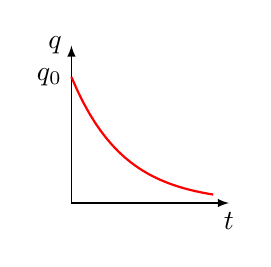
\begin{tikzpicture}[>=latex]
					\draw[->] (0,0) -- ++(2,0) node[below] {$t$};
					\draw[->] (0,0) -- ++(0,2) node[left] {$q$};
					\node[left] at (0, 1.6) {$q_0$};
					\draw[domain=0:1.8, red, thick] plot (\x, {1.6*exp(-1.5*\x)});
				\end{tikzpicture}
			\end{column}
			\begin{column}{0.7\linewidth}
				\begin{block}{}
					Закон Ома для кола $RI = U$. Оскільки $I = -dq/dt$ і $U= q/C$, закон набуде вигляду
					\begin{equation*}
						\frac{dq}{dt}  + \frac{q}{RC} = 0.
					\end{equation*}
					Після інтегрування ми отримаємо:
					\begin{equation*}
						q = q_0e^{-t/RC } = q_0e^{- t / \tau},
					\end{equation*}
					де $q_0$ --- початковий заряд конденсатора, а $\tau = RC$ --- називають \alert{часом релаксації}.
				\end{block}
			\end{column}
		\end{columns}
	\end{onlyenv}
	\framesubtitle<3>{Зарядка конденсатора}
	\begin{onlyenv}<3>
		\begin{columns}
			\begin{column}{0.3\linewidth}\centering
				\begin{circuitikz}[european, scale=0.7, transform shape]
					\draw
					(0,0) to[battery2, l=$\mathcal{E}$] ++(0,2)  to[R, l=$R$] ++(2.5, 0) to[C, l=$C$] ++(0, -2)
					to[opening switch, l=$S$, mirror] ++(-2.5, 0) -- cycle
					;
				\end{circuitikz}
				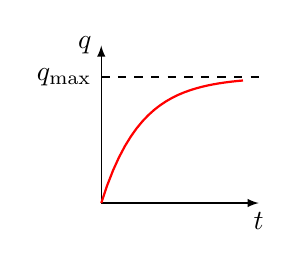
\begin{tikzpicture}[>=latex]
					\draw[->] (0,0) -- ++(2,0) node[below] {$t$};
					\draw[->] (0,0) -- ++(0,2) node[left] {$q$};
					\node[left] at (0, 1.6) {$q_{\max}$};
					\draw[dashed] (0, 1.6) -- ++(2,0);
					\draw[domain=0:1.8, red, thick] plot (\x, {1.6*(1-exp(-2*\x))});
				\end{tikzpicture}
			\end{column}
			\begin{column}{0.7\linewidth}
				\begin{block}{}
					Закон Ома для кола $RI + U = \mathcal{E}$. Оскільки $I = dq/dt$ і $U= q/C$, закон набуде вигляду
					\begin{equation*}
						\frac{dq}{dt}  + \frac{q}{RC} =  \mathcal{E}.
					\end{equation*}
					Після інтегрування ми отримаємо:
					\begin{equation*}
						q =  q_{\max}(1 - e^{- t / \tau}),
					\end{equation*}
					де $q_{\max} = \mathcal{E} C$ --- граничне значення заряду на конденсаторі ($t \to \infty$).
				\end{block}
			\end{column}
		\end{columns}
	\end{onlyenv}
\end{frame}
% ===========================================================================



% ============================== Слайд ## ===================================
\begin{frame}{Підсумки}{}\small
	\begin{overprint}
		\onslide<1>
		\begin{tblr}{colspec={Q[l,m]Q[l,m,mode=dmath]}}
			Сила струму                                      & I = \frac{dq}{dt}                                                              \\
			Вектор густини струму                            & j = \frac{dI}{dS_{\perp}}                                                      \\
			Струм, як потік вектора $\vect{j}$               & I = \iint\limits_S \vect{j}\cdot d\vect{S}                                     \\
			Зв'язок густини струму і густини заряду          & \vect{j} = \rho\vect{u}                                                        \\
			Закон збереження заряду (рівняння неперервності) & \Div\vect{j} = - \frac{\partial\rho}{\partial t}                               \\
			Закон Ома в інтегральній формі                   & I = \frac{U}{R}                                                                \\
			Закон Ома в диференціальній формі                & \vect{j} = \lambda\Efield                                                      \\
			Провідність металів за теорією Друде             & \lambda = \frac{ne^2\tau}{2m_e}                                                \\
			Електрорушійна сила (означення)                  & \mathcal{E} = \frac{A^*}{q} = \int\limits_{(1)}^{(2)}\vect{E}^*\cdot d\vect{r}
		\end{tblr}
		\onslide<2>
		\begin{tblr}{colspec={Q[l,m]Q[l,m,mode=dmath]}}
			Електрорушійна сила (означення)              & \mathcal{E} = \frac{A^*}{q} = \int\limits_{(1)}^{(2)}\vect{E}^*\cdot d\vect{r} \\
			Закон Ома для неоднорідної ділянки кола      & IR = \phi_1 - \phi_2 + \mathcal{E}                                             \\
			Перше правило Кірхгофа (для вузла)           & \sum\limits_{k=1}^{K} I_k = 0                                                  \\
			Друге правило Кірхгофа (для контурів)        & \sum\limits_{m=1}^{M} I_m R_m = \sum\limits_{n=1}^{N} \mathcal{E}              \\
			Закон Джоуля-Ленца (в диференціальній формі) & w = \lambda E^2                                                                \\
			Закон Джоуля-Ленца (в Інтегральній формі)    & W = I R^2
		\end{tblr}
	\end{overprint}
\end{frame}
% ===========================================================================


\end{document}
